
\begin{figure}[htbp]
\centering
 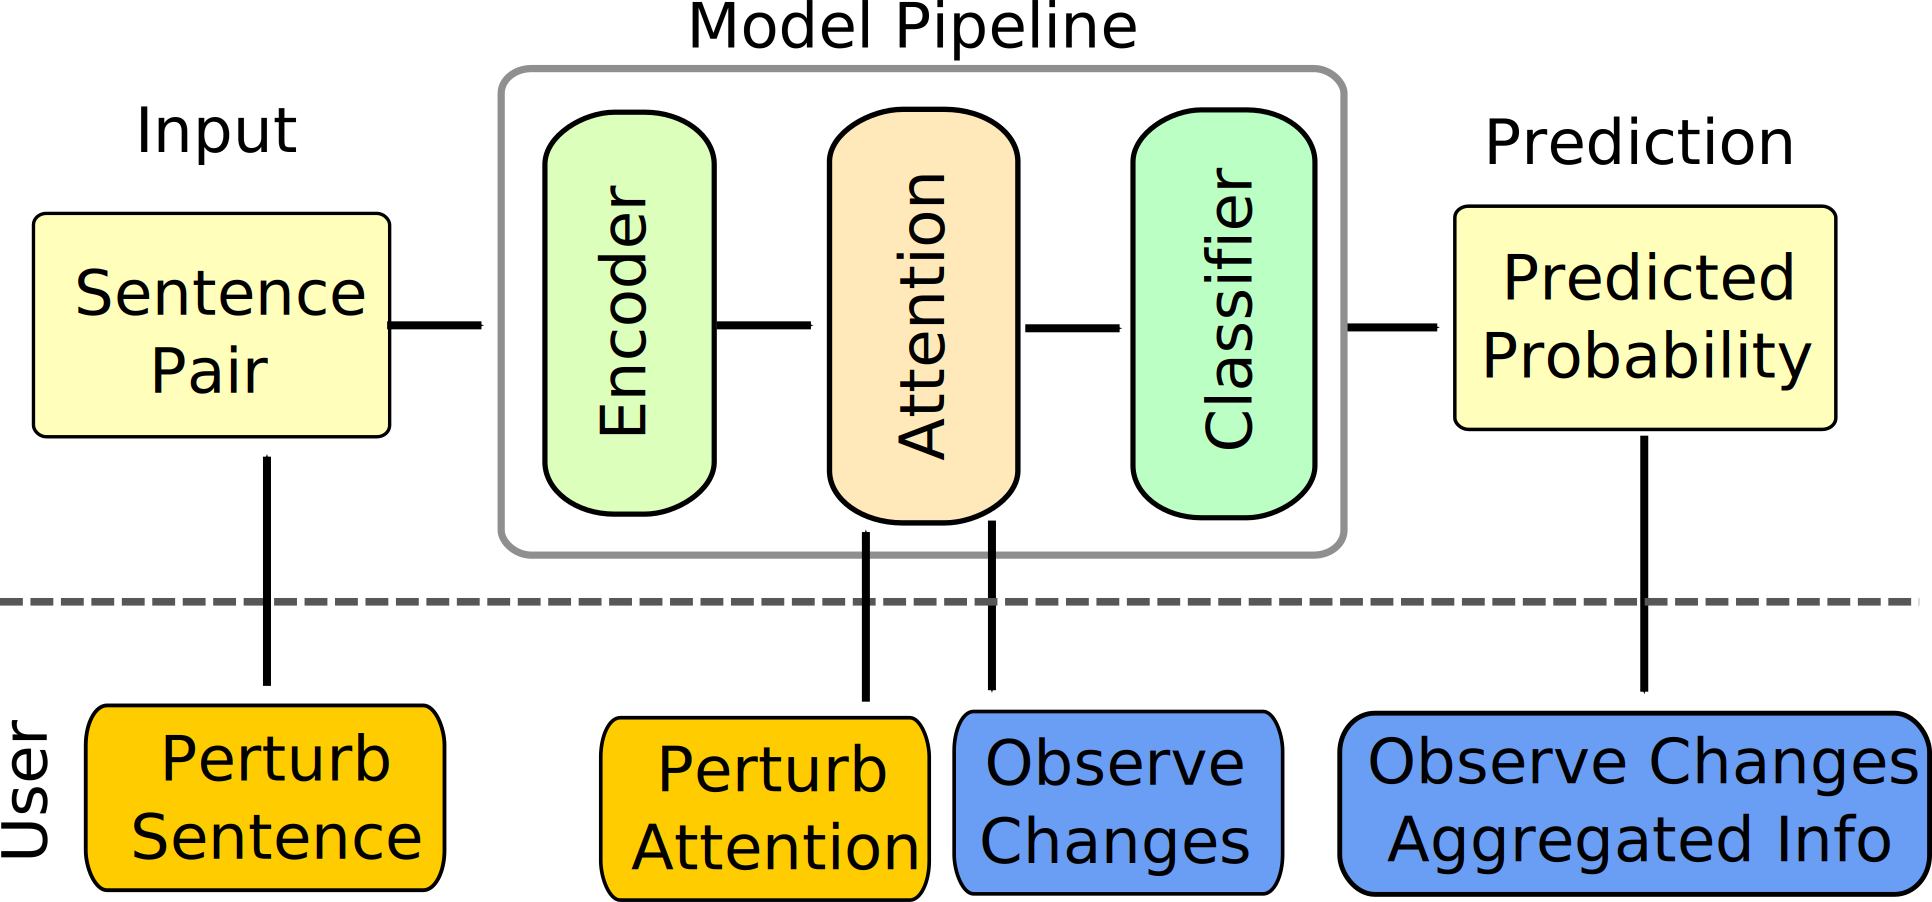
\includegraphics[width=1.0\linewidth]{pipeline}
 \caption{
Perturbation-driven exploration of the natural language inference model.
In the proposed tool, we enables the automated or user-guided perturbation of the input sentence (e.g., replace words), the attention in the model (e.g., alter the alignment between sentences), and the prediction (e.g., adjust the prediction by making updates to the model).
}
\label{fig:modelPipeline}
\end{figure}

\section{NLIZE System}
In this section, we describe the design and implementation of the NLIZE (pronounced as ``analyze'') system, which address the analysis tasks (T1-3).
%
As discussed in the task analysis, the experts obtain intuition about the model via guided exploration by studying how various parts of the pipeline behave when certain components are altered.
%
This can be generalized as the perturbation-driven paradigm, which formulated the basic guiding principal for designing the proposed tool.
As illustrated in Fig.~\ref{fig:modelPipeline}, we enables the automated or user-guided perturbation of the input sentence (e.g., replace words), the attention in the model (e.g., alter the alignment between sentences), and the prediction (e.g., adjust the prediction by making updates to the model).
%
In the following sections, we describe in detail the five major components of the proposed system, namely, all pair summary view, sentence view, attention view, prediction view, pipeline view.


% Beside looking into the internal states, understanding how each of the component of the model interact with input and output as well as with each other is the crucial for truly examine the mechanism of the model.
%
% Look at how the model work in action and interrogate relationship between different component, i.e., how the change made to one part of model affect the other pieces present, is the key to gain the full picture.
